
Alguns pesquisadores, como \citeonline{Suresh2012}, tentaram mapear elementos essenciais e como interagem entre si para que um determinado Ecossistema possa crescer.
 \citeonline{Lemos2011} diz que pesquisas sobre ecossistemas de empreendedorismo apresentam um forte caráter exploratório e que faltam teorias consolidadas sobre as relações entre os diversos elementos que compõem um ecossistema. 
 \citeonline{marmer2011startup}, por meio do Startup Genome, organização sem fins lucrativos que realiza análises de Ecossistemas de Startups em todo o mundo entrevistou cerca de 11 mil empreendedores em 40 ecossistemas e dividiu o ciclo de vida de uma Startup em seis estágios: a Descoberta, a Validação, a Eficiência, a Escala, a Sustentabilidade e a fase de Conservação. 

 Como um dos resultados dessa pesquisa descobriram a grande importância que esse ciclo possui nas chances de sucesso de uma Startup, de forma que aquelas que cresceram de forma muito acelerada e inconsistente, sem respeitar o desenvolvimento de todas as fases do ciclo e suas capacidades, obtiveram resultados muito inferiores, como representado na figura \ref{figure:valuation_ao_escalar}. \citeonline{Moore2014} diz que durante o ``Vale da Morte'' é muito importante que a empresa atinga um certo nível de maturidade para conseguir superar essa fase, enfatizando, também, a importância de não pular etapas no desenvolvimento de uma Startup.

\chapter[Sobre Ecossistemas de Startups]{Sobre Ecossistemas de Startups}
\label{cap-sobre-ecossistemas-de-startups}

\citeonline{Unterkalmsteiner2016} relatam que uma das áreas de pesquisa de maior importância acerca de startups envolve o estudo de ecossistemas, em especial estudos que busquem responder perguntas a respeito dos elementos chaves de um ecossistema frutífero, os tipos de ecossistemas (diferentes tamanhos, nichos de mercado e tecnologia, etc), como eles evoluem com o passar do tempo e técnicas de como mensurar a qualidade de um determinado ecossistema de startups. \citeonline{Lemos2011} diz que pesquisas sobre ecossistemas de empreendedorismo apresentam um forte caráter exploratório e que faltam teorias consolidadas sobre as relações entre os diversos elementos que compõem um ecossistema, trabalho que diversos autores vem tentando conduzir nos últimos anos.

\citeonline{Arnaud2009} e \citeonline{Ahmad2007}, por exemplo, apresentaram uma abordagem para avaliação de ecossistemas concentrada em três grandes pilares: 1) Fatores Determinantes, envolvendo indicadores de ambiente regulatório, acesso a capital, cultura e capacidades empreendedoras; 2) Performance, englobando indicadores relativos as empresas da região; e 3) Impacto, envolvendo indicadores sociais como índices de geração de empregos, crescimento econômico e redução da pobreza. 

\citeonline{Hermann2015}, por meio do ``The Global Startup Ecosystem Ranking'' e da Compass, realizaram um estudo sobre ecossistemas com base em seis pilares principais: Performance, Financiamento, Alcance de Mercado, Talento, Experiência em Startups e Índice de Crescimento. 

A \citeonline{indiceglobaldoempreendedorismo}, que anualmente publica o Índice de Cidades Empreendedoras, tem sua análise de ecossistemas baseada em sete pilares: ambiente regulatório, infraestrutura, mercado, acesso a capital, inovação, capital humano e cultura empreendedora. De acordo com a Endeavor, entre os anos de 2015 e 2016, Brasília demonstrou uma melhora significativa em alguns dos pilares mas, também, piora em outras, como demonstrado pela Figura \ref{figure:ici20152016}.

\begin{figure}[!htb]
	\centering
	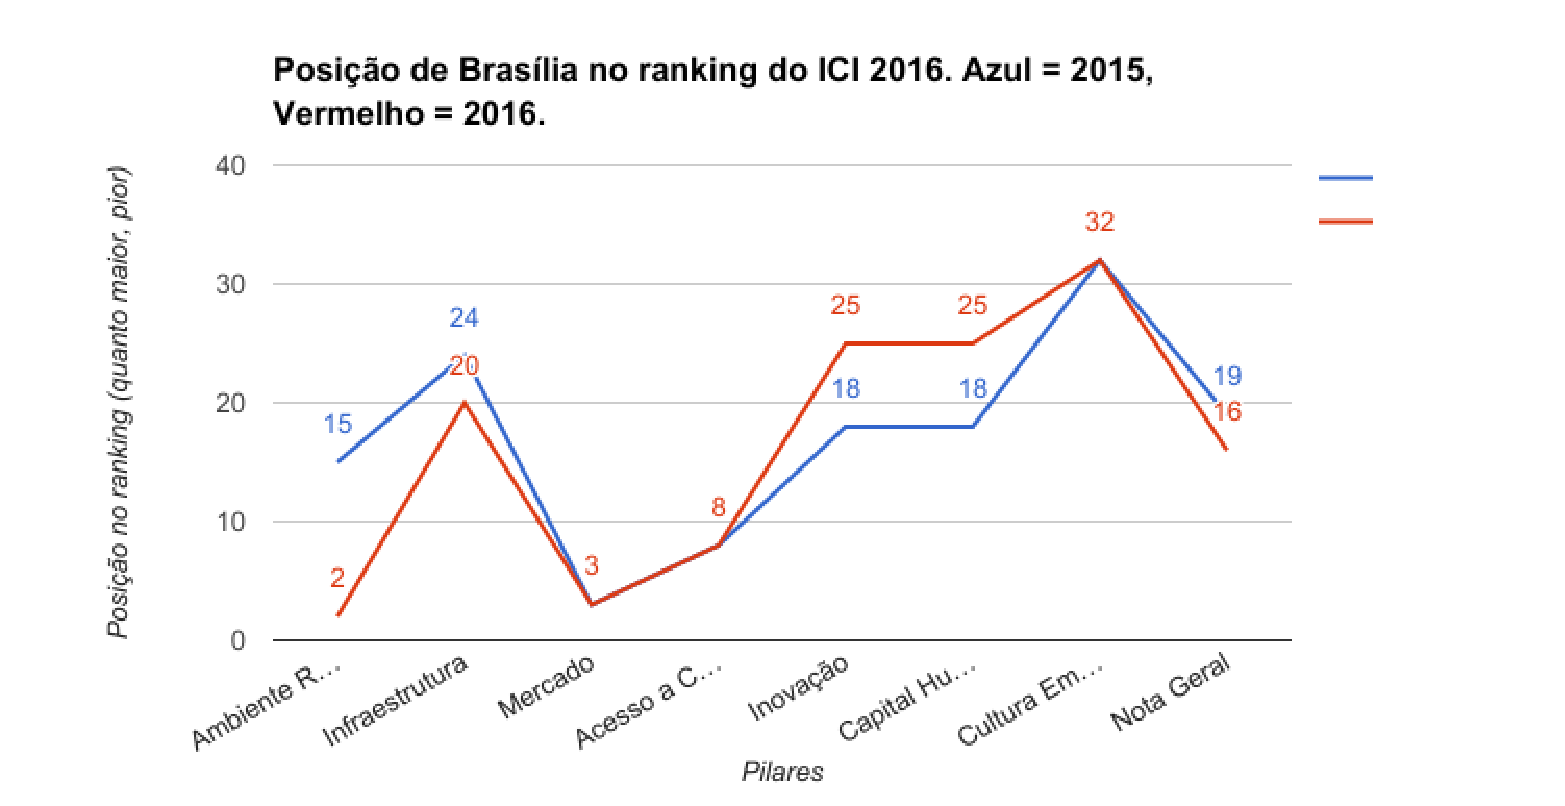
\includegraphics[width=11cm,angle=0]{figuras/ici20152016}
	\caption{Comparação dos indicadores de Brasília no Índice de Cidades Empreendedoras entre os anos 2015 e 2016}
	\label{figure:ici20152016}
\end{figure}

\citeonline{Suresh2012}, por exemplo, concentrou seus trabalhos em mapear os elementos de um ecossistema que contribuem para a formação do indivíduo empreendedor como a presença de suporte de uma rede que apoie o empreendedor nos momentos difíceis e sirva de exemplo para o mesmo como referências de sucesso. 

\citeonline{Arnaud2009} e \citeonline{Ahmad2007} por meio da OECD definiram três grandes pilares para avaliar o Empreendedorismo em uma região. O primeiro, de Determinantes, é composto por indicadores Ambiente Regulatório, Cultura, Pesquisa \& Desenvolvimento e Tecnologia, Acesso à Financiamento, Capacidades Empreendedoras, Condições do Mercado. O segundo pilar, chamado de Performance Empreendedora, é composto por indicadores baseados nas empresas e nos empregos da região. O terceiro, de Impacto, estuda dados comos Criação de Empregos, Crescimento Econômico e Redução da Pobreza. No mesmo artigo são indicados diversas fontes e meios para se obter dados sobre esses indicadores.



\citeonline{Spigel2015} diz que o estudo de ecossistemas empreendedores se tornaram uma ferramenta popular para o estudo do empreendedorismo de alto crescimento sob o ponto de vista geográfico. 

\section{O Dinâmico Mercado de Startups e de Investidores}
\label{section:o_dinamico_mercado_das_startups}

\section{O Ecossistema}
\label{section:ecossistemas_e_suas_pecas}

\citeonline{James1953} diz que o crescimento econômico, a formação e o crescimento de cidades está diretamente ligado ao empreendedorismo e as decisões que são tomadas por empreendedores. \citeonline{Dalcin2015} relata que alguns dos impactos locais de um bom Ecossistema de Startups envolvem a criação de empregos, o crescimento econômico e a redução da pobreza. 

\citeonline{Schumpeter1934} diz que empreendedores tendem a se conglomerar em uma mesmo região com o objetivo de obterem benefícios mútuos, criando clusters, que podem ser interpretados como Ecossistemas, e são essenciais para o desenvolvimento local.

\citeonline{Dubini1989} diz que ecossistemas são marcados pela presença de empresas, uma economia diversificada, uma boa infraestrutura de negócios e investimentos, uma cultura adequada e políticas públicas que apoiem os Empreendedores e a criação de novos empreendimentos. \citeonline{ranga2013triple} trás uma abordagem com o conceito da Hélice Tripla, que representa a interação entre Governo, Indústria e Academia, como representado pela Figura \ref{figure:triple_helix}. 

\begin{figure}[!htb]
\centering
\includegraphics[width=11cm,angle=0]{figuras/triple_helix}
\caption{Modelo de Hélice Tripla, por \citeonline{ranga2013triple}}
\label{figure:triple_helix}
\end{figure}

\citeonline{isenberg2011introducing} mapeia os Ecossistemas Empreendedores em seis grandes pilares: Política, Finanças, Cultura, Suporte, Capital Humano e Mercado, onde todos devem agir em conjunto para a criação de um Ecossistema saudável e promissor. Essa visão está representada na Figura \ref{figure:isenberg_ecosystem}. \citeonline{schwab2015} defende que os pilares são Abertura de Mercados, Capital Humano, Investimento, Apoio do Governo, Ambiente Regulatório, Educação, Universidades e Suporte Cultural.

\begin{figure}[!htb]
\centering
\includegraphics[width=11cm,angle=0]{figuras/isenberg_ecosystem}
\caption{Ecossistemas Empreendedores, por \citeonline{isenberg2011introducing}}
\label{figure:isenberg_ecosystem}
\end{figure}

\citeonline{gumpert1985heart} diz que enquanto o Governo e a Academia podem criar condições favoráveis para que o empreendedorismo aconteça o envolvimento de indivíduos é essencial, reforçando o modelo criado por Isenberg e indo contra o conceito da Hélice Tripla.

\citeonline{Stangler2015}, por meio da Kauffman Foundation, definem os quatro seguintes indicadores de um Ecossistema vibrante: Densidade, Fluídez, Conectividade e Diversidade. Para o indicador Densidade, eles sugerem que medidas indicadas podem ser a quantidade de novas empresas para cada mil pessoas, a quantidade de emprego nessas empresas e a densidade dos setores, em especial que envolvam alta tecnologia. Para Fluídez indicam o fluxo populacional de uma cidade, a realocação no mercado de trabalho e a quantidade de empresas de alto crescimento. Para se medir Conectividade os dados podem ser relacionados à redes de investidores, conectividade entre programas e a quantidade de spin-offs. Por fim, diversidade idealmente pode ser medida pela quantidade de especializações econômicas, taxa de mobilidade e de imigrantes. O artigo em si não descreve um arcabouço para avaliação de Ecossistemas, mas define bons quatro indicadores que podem ser utilizados por outros trabalhos, por este, inclusive. 

\citeonline{Motoyama2014}, também por intermédio da Kauffman Foundation, identificaram quatro pontos de conexão chave em um ecossistema empreendedor e os dividiram em quatro níveis: Conexões entre Empreendedores, Conexões entre Organizações de Suporte, Conexões entre Empreendedores e Organizações de Suporte e Conexões de Suporte Diversas, como eventos. Esses conceitos foram de extrema importância para este Trabalho, visto que é muito claro que são essas Conexões que movem o Ecossistema.

\citeonline{Spigel2015} define Ecossistemas como a união entre elementos culturais, sociais, políticos e econômicos em uma região que propíciam o crescimento de empresas inovadoras e encorajam novos empreendedores e outros atores a assumirem os riscos relacionados a essas empresas. Com um extenso estudo o autor construiu a Tabela \ref{table:attributes_of_entrepreneurship_ecosystems} com os atributos de ecossistemas empreendedores, ele também criou uma pirâmide que representa as relações entre esses atributos, representado pela Figura XX.

\begin{table}[!htb]
	\centering
	\begin{tabular}{ | p{3cm} | p{4cm} | p{8cm} | }
		\hline
		Tipo & Atributo & Descrição \\ \hline
		Cultura & Apoio & Atitudes culturais que apoiam e transformam atividades empreendedoras, risco e inovação em situações normais. \\ \hline
		Cultura & Histórias de Empreendedorismo & Exemplos locais de empresas e empreendedores de sucesso. \\ \hline
		Social & Talento & Presença de profissionais talentosos e experientes dispostos a trabalhar em startups. \\ \hline
		Social & Investimento & Disponibilidade de capital para investimento de famílias e amigos, investidores anjos e venture capital. \\ \hline
		Social & Redes & Presença de redes sociais que conectem empreendedores, conselheiros, investidores e profissionais que permitam o fluxo livre de conhecimento e experiências. \\ \hline
		Social & Mentores & Empreendedores e profissionais locais bem sucedidos dispostos a contribuir com o crescimento de jovens empreendedores. \\ \hline
		Material & Políticas Públicas & Programas estatais e regulamentações que apoiem o Empreendedorismo ou removam barreiras para a criação de novas empresas. \\ \hline
		Material & Universidades & Universidades e outras instituições educacionais que preparam novos Empreendedores e produzem conhecimento relevante para o Ecossistema. \\ \hline
		Material & Serviços de Suporte & Organizações especializadas em oferecer suporte para novas empresas como advogados, incubadoras, contadores, etc. \\ \hline
		Material & Infraestrutura & Disponibilidade de espaços para escritórios, acesso a recursos de telecomunicação e transporte, etc. \\ \hline
		Material & Abertura de Mercado & Presença de oportunidades locais que permitam que as empresas creçam de forma global. \\ \hline
	\end{tabular}
	\caption{Atributos de Ecossistemas Empreendedores, por \cite{Spigel2015}}
	\label{table:attributes_of_entrepreneurship_ecosystems}
\end{table}

\begin{figure}[!htb]
\centering
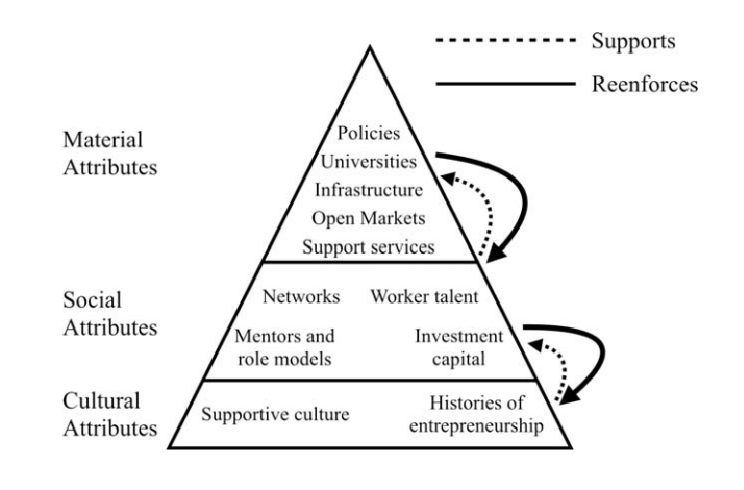
\includegraphics[width=11cm,angle=0]{figuras/relationship_among_ecosystems_attributes}
\caption{Relacionamentos entre atributos de Ecossistemas Empreendedores, por \citeonline{Spigel2015}}
\label{figure:relationship_among_ecosystems_attributes}
\end{figure}

\citeonline{Coutu2014} criou um relatório em que sugere seis áreas que atores de um Ecossistema - como governos, universidades, corporações e mídia - podem concentrar ações de forma a criar um bom ambiente para que as startups cresçam, bem como ações que podem ser tomadas de acordo com a visão dos empreendedores e líderes de startups entrevistados. Essas áreas exploradas pelo relatório são as seguintes:

\begin{description}
	\item [Definição de metas, apoio, promoção e informações sobre Startups:] a autora diz que a ação mais importante que governos podem fazer para apoiar o crescimento das Startups é liberar dados que permitam quaisquer interessados na economia local identificarem quais são essas empresas que tanto crescem e a segunda ação mais importante seria a colaboração com aqueles atores, sejam públicos ou privados, que já estão ou querem apoiar Startups. 

	\item [Acesso a talentos:] para muitos líderes e empreendedores o maior empecilho para o crescimento de suas organizações é o acesso à profissionais capacitados, a talentos. 

	\item [Desenvolvimento de lideranças:] o segundo maior empecilho para esses líderes e empreendedores é a falta de profissionais de nível senior com experiência e capacidade para liderar times, eles alegam que é difícil fazer uma empresa crescer dezenas ou centenas de vezes mais rápido do que o normal, como acontece com as Startups, sem um bom time.

	\item [Aumento da quantidade de vendas locais e internacionais:] existem muitas barreiras que dificultam a criação de novos produtos e serviços para mercados, tanto internacionais quanto locais ou domésticos.

	\item [Investimento para Startups:] a autora relata que é comum que Startups busquem investimento nos Estados Unidos da América ou em países da Ásia por existirem diversos mecânismos de suporte para essas empresas, que por fim acabam não deixando o país. Para que elas não saiam, ou sejam vendidas para investidores de outros países, os atores locais precisam criar ambientes atrativos para que as Startups não busquem recursos em outras regiões.

	\item [Acesso a infraestrutura:] a falta de infraestrutura adequada pode fazer com que seja mais difícil para que uma Startup escale do que seria em um Ecossistema adequado. A falta de infraestrutura pode estar relacionada tanto ao Ambiente Regulatório como também a dificuldade para se conseguir um espaço físico ou recursos de comunicação, como internet de boa qualidade.

\end{description}


\citeonline{Feld2012}, empreendedor bem sucedido e um especialista em Ecossistemas de Startups, contribuiu a ``Teoria de Boulder'' em que ele define quatro regras para um bom Ecossistema: 1) Precisa ser liderado por Empreendedores; 2) Os líderes precisam assumir um compromisso a longo prazo para com o Ecossistema; 3) O Ecossistema precisa ser inclusivo para qualquer pessoa que queira participar; 4) O Ecossistema precisa ter atividades contínuas que engajem toda a comunidade empreendedora local. Ele também elencou alguns atores que compõem e são de grande importância para ecossistemas como empreendedores, Governo, Universidades, Investidores, Mentores, Provedores de Serviço e Grandes Empresas. Outro fator interessante é que ele enxerga Ecossistemas Empreendedores como organismos que estão em constante evolução, e não estruturas bem definidas. Com base nesse princípio ele também faz a divisão de atores entre ``semeadores'' (seeders, aqueles que fomentam e criam o movimento no Ecossistema) e ``alimentadores'' (feeders, todos aqueles que não atuam como semeadores e se beneficiam do crescimento do Ecossistema). 

\citeonline{Stam2015} fez uma ótima síntese dos atributos de um bom Ecossistema que foram explorados no livro ``Startup Communities'' de Feld, exibido pela Tabela \ref{table:attributes_of_entrepreneurship_ecosystems}, e \citeonline{Chua2012} criou um ótimo rascunho sobre o mesmo livro, exibido pela Figura \ref{figure:startup_communities}.

\begin{table}[!htb]
	\centering
	\begin{tabular}{ | p{3cm} | p{12cm} | }
		\hline
		Atributo & Descrição \\ \hline
		Liderança & Grupo forte de empreendedores que são bem conhecidos no Ecossistema, acessíveis e compromissados com o desenvolvimento local da região. \\ \hline
		Intermediários & Mentores e conselheiros bem respeitados que contribuam com o Ecossistema, aceleradoras e incubadoras também podem tomar esse papel. \\ \hline
		Densidade da Rede & Uma comunidade de empreendedores bem sucedidos e muito bem conectados com investidores, mentores, conselheiros, apoiadores, etc. Todos devem estar dispostos a dar mais do que receber do Ecossistema. \\ \hline
		Governo & Forte apoio do governo tanto em ajudar como em entender o contexto das Startups e em como alterar o ambiente regulatório de forma a contribuir com o desenvolvimento de mais empresas. \\ \hline
		Talentos & Diversas opções de talentos com diferentes níveis de experiência e conhecimento disponíveis no mercado local para empresas de todos os tamanhos e estágios em todas as áreas do conhecimento. Boa parte desses profissionais vem da universidade e por isso devem estar bem conectadas com o Ecossistema. \\ \hline
		Apoiadores & Advogados, contadores, etc integrados, acessíveis, efetivos e com uma oferta de serviços com preços adequados. \\ \hline
		Engajamento & Um grande número de eventos para que Empreendedores e Ecossistema se conectem. Podem ser meetups, dias de pitch, hackathons, startup weekends, etc. \\ \hline
		Empresas & Grandes empresas estabelecidas podem ter um grande papel como apoiadores das novas Startups, seja fornecendo infraestrutura, conhecimento ou investimento que os Empreendedores possam utilizar. \\ \hline
		Capital &  Uma comunidade forte, apoiadora e presente de investidores dos mais diversos tipos como anjos, venture capital, etc. \\ \hline
	\end{tabular}
	\caption{Atributos de um Ecossistema de Startups bem sucedido, por \cite{Stam2015} e \cite{Feld2012}}
	\label{table:attributes_of_entrepreneurship_ecosystems}
\end{table}

\begin{figure}[!htb]
\centering
\includegraphics[width=11cm,angle=0]{figuras/startup_communities}
\caption{Rascunho, criado por \citeonline{Chua2012}, sobre o livro ``Startup Communities'', criado por {Feld2012}}
\label{figure:startup_communities}
\end{figure}